\documentclass[11pt, a4paper]{article}

\usepackage[utf8]{inputenc}
\usepackage[left=2cm,text={17cm, 24cm},top=3cm]{geometry}

\usepackage{times}
\usepackage[unicode]{hyperref}
\usepackage{multirow}
\usepackage{amssymb}
\usepackage{graphics}
\usepackage[ruled, czech, noline, linesnumbered, longend]{algorithm2e}
\usepackage{pdflscape}
\usepackage[czech]{babel}
\urlstyle{rm}

\begin{document}

\begin{titlepage}
\begin{center}

\Huge
\textsc {Vysoké učení technické v~Brně}\\

\huge
\textsc {Fakulta informačních technologií}\\
\vspace{\stretch{0.382}}
    \LARGE {Typografie a~publikování\,--\,3. projekt}\\
    \Huge {Tabulky a obrázky}
\vspace{\stretch{0.618}}
\end{center}


{\Large
3. dubna 2021
\hfill Lenka Šoková }
\end{titlepage}

\section{Úvodní strana}
Název práce umístěte do zlatého řezu a nezapomeňte uvést dnešní datum a vaše jméno a příjmení.

\section{Tabulky}
Pro sázení tabulek můžeme použít buď prostředí\texttt{ tabbing }nebo prostředí\texttt{ tabular}.

\subsection{Prostředí\texttt{ tabbing}}
Při použití\texttt{ tabbing }vypadá tabulka následovně:
\begin{tabbing}
\textbf{Ovoce}\hspace{0.71in}\=\textbf{Cena}\hspace{0.20in}\=\textbf{Množství}\\ %TODO
Jablka \> 25,90 \> 3 kg\\
Hrušky \> 27,40 \> 2,5 kg\\
Vodní melouny \> 35,-- \> 1 kus\\
\end{tabbing}

\noindent
Toto prostředí se dá také použít pro sázení algoritmů, ovšem vhodnější je použít 
prostředí\texttt{ algorithm }nebo\texttt{ algorithm2e }(viz sekce \ref{alg:sec}).

\subsection{Prostředí\texttt{ tabular}}
Další možností, jak vytvořit tabulku, je použít prostředí\texttt{ tabular}. Tabulky pak budou vypadat takto\footnote{Kdyby byl problem s\texttt{ cline,} zkuste sa podívat třeba sem: \url{http://www.abclinuxu.cz/tex/poradna/show/325037}.}:
\bigskip

\begin{table}[h]
\centering
\catcode`\-=12

\begin{tabular}{|l|c|c|} 
    \hline
    & \multicolumn{2}{c|}{\textbf{Cena}}\\\cline{2-3}
    \textbf{Měna} & \textbf{nákup} & \textbf{prodej}\\
    \hline
    EUR & 25,227 & 26,943\\
    GBP & 29,368 & 31,492\\
    USD & 21,260 & 22,661\\
    \hline
\end{tabular}
\caption{Tabuľka kurzů k~dnešnímu dni}
\label{tab:kurz}
\end{table}
\bigskip

\begin{table}[h] 
\centering 
\catcode`\-=12

\begin{tabular}{|c|c|} 
\hline
$A$ & $\neg A$\\ \hline
\textbf{P} & N \\ \hline
\textbf{O} & O \\ \hline
\textbf{X} & X \\ \hline
\textbf{N} & P \\ \hline
\end{tabular}
\begin{tabular}{|c|c|c|c|c|c|}
\hline
\multicolumn{2}{|c|}{\multirow{2}{*}{$A \wedge B$}} & \multicolumn{4}{c|}{$B$}\\ \cline{3-6}
\multicolumn{2}{|c|}{}& \textbf{P} & \textbf{O} & \textbf{X} & \textbf{N} \\\hline \cline{2-6}
\multirow{4}{*}{$A$}& \textbf{P} & P & O & X & N \\\cline{2-6}
& \textbf{O} & O & O & N & N \\\cline{2-6}
& \textbf{X} & X & N & X & N \\ \cline{2-6}
& \textbf{N} & N & N & N & N \\ \hline
\end{tabular}
\begin{tabular}{|c|c|c|c|c|c|}
\hline
\multicolumn{2}{|c|}{\multirow{2}{*}{$A \vee B$}} & \multicolumn{4}{c|}{$B$}\\ \cline{3-6}
\multicolumn{2}{|c|}{}& \textbf{P} & \textbf{O} & \textbf{X} & \textbf{N} \\\hline \cline{2-6}
\multirow{4}{*}{$A$}& \textbf{P} & P & O & X & N \\\cline{2-6}
& \textbf{O} & O & O & N & N \\\cline{2-6}
& \textbf{X} & X & N & X & N \\ \cline{2-6}
& \textbf{N} & N & N & N & N \\ \hline
\end{tabular}
\begin{tabular}{|c|c|c|c|c|c|}
\hline
\multicolumn{2}{|c|}{\multirow{2}{*}{$A \rightarrow B$}} & \multicolumn{4}{c|}{$B$}\\ \cline{3-6}
\multicolumn{2}{|c|}{}&\textbf{P} & \textbf{O} & \textbf{X} & \textbf{N} \\\hline \cline{2-6}
\multirow{4}{*}{$A$}& \textbf{P} & P & O & X & N \\\cline{2-6}
& \textbf{O} & O & O & N & N \\\cline{2-6}
& \textbf{X} & X & N & X & N \\ \cline{2-6}
& \textbf{N} & N & N & N & N \\ \hline
\end{tabular}
\caption{Protože Kleeneho trojhodnotová logika už je \uv{zastaralá}, uvádíme si zde pŕíklad čtyřhodnotové logiky}
\label{tab:logika}
\end{table}
\bigskip
\section{Algoritmy} \label{alg:sec}
Pokud budeme chtít vysázet algoritmus, můžeme použít prostředí\texttt{ algorithm\footnote{Pro nápovědu, jak zacházet s~prostředím\texttt{ algorithm, }můžeme zkusit tuhle stránku:\\\url{http://ftp.cstug.cz/pub/tex/CTAN/macros/latex/contrib/algorithms/algorithms.pdf}.} }nebo\texttt{ algorithm2e}\footnote{Pro\texttt{ algorithm2e }zase tuhle: \url{http://ftp.cstug.cz/pub/tex/CTAN/macros/latex/contrib/algorithm2e/doc/algorithm2e.pdf}.}.\\
Příklad použití prostředí\texttt{ algorithm2e }viz Algoritmus \ref{alg:FastSLAM}.

\vspace{7mm}
\begin{algorithm}[H] \label{alg:FastSLAM}
\caption{\textsc{FastSLAM}}
%\SetNlSkip{-1.2em}
\SetNlSkip{-1.2em}
\SetInd{1em}{1em}
\SetNlSty{}{}{:}
\SetAlgoNlRelativeSize{-1}

\KwIn{ $(X_{t-1}, u_t, z_t)$ }
\KwOut{ $X_t$ }
\Indp\Indpp
\BlankLine

$\overline{X_t} = X_t = 0$\\
\For{$ k = 1 \emph{ to } M$}{
$x_t^{[k]} = \emph{sample\_motion\_model}(u_t, x_{t-1}^{[k]})$\\
$w_t^{[k]} = \emph{measurement\_model}(z_t, x_t^{[k]}, m_{t-1})$\\
$m_t^{[k]} = updated\_occupancy\_grid(z_t, x_t^{[k]}, m_{t-1}^{[k]})$\\
$\overline {X_{t}} = \overline {X_{t}} + \langle x_x^{[k]}, m_t^{[k]}\rangle$\\}

\For{$ k = 1 \emph{ to } M$}{
draw $i$ with probability $\approx \omega_t^{[i]}$\\
add $\langle x_x^{[k]}, m_t^{[k]}\rangle$ to $X_t$}

\KwRet{$X_t$}
\end{algorithm}
\bigskip


\section{Obrázky}
Do našich článků můžeme samozřejmě vkládat obrázky. Pokud je obrázkem fotografie,
můžeme klidně použít bitmapový soubor. Pokud by to ale mělo být nějaké schéma nebo
něco podobného, je dobrým zvykem takovýto obrázek vytvořit vektorově.

\begin{figure}[ht]
    \centering
    \scalebox{0.40}{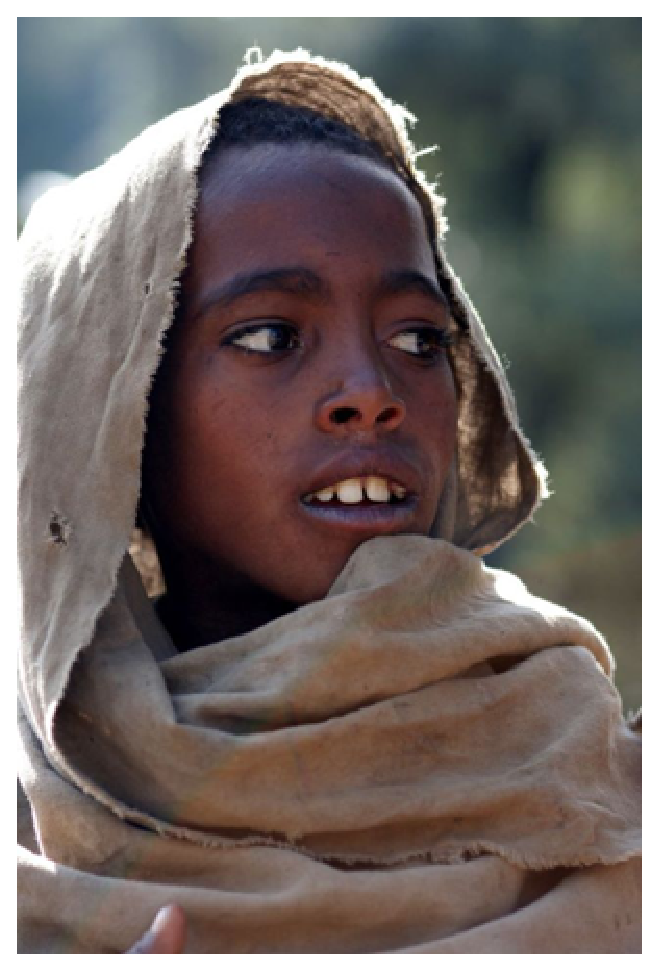
\includegraphics{etiopan.eps}
    \hspace{-0.4em}
    \reflectbox{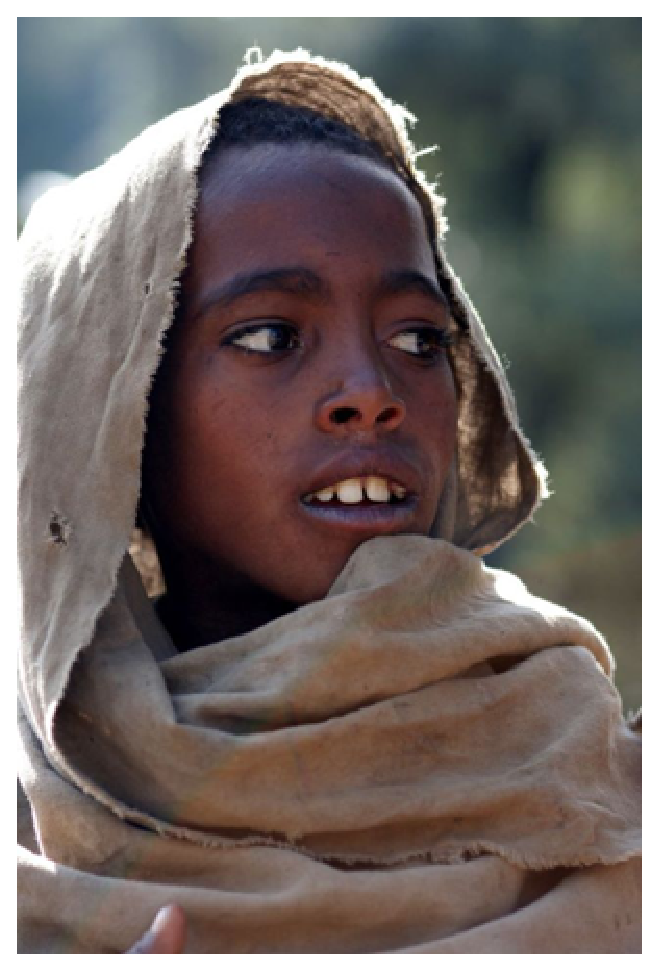
\includegraphics{etiopan.eps}}}
    \caption{Malý Etiopánek a jeho bratříček}
    \label{fig:Etiopan}
\end{figure}
\newpage

Rozdíl mezi vektorovým\,\dots \par
\begin{figure}[ht]
    \centering
    \scalebox{0.40}{
\includegraphics{oniisan.eps}}
    \caption{Vektorový obrázek}
    \label{fig:vector}
\end{figure}
\noindent
\\\dots\,a bitmapovým obrázkem \par
\begin{figure}[ht]
    \centering
    \scalebox{0.60}{
\includegraphics{oniisan2.eps}}
    \caption{Bitmapový obrázek}
    \label{fig:bitmap}
\end{figure}

\noindent
\\se projeví například při zvětšení.

Odkazy (nejen ty) na obrázky \ref{fig:Etiopan}, \ref{fig:vector} a \ref{fig:bitmap}, na tabulky \ref{tab:kurz} a \ref{tab:logika} a také na algoritmus \ref{alg:FastSLAM} jsou udělány pomocí křížových odkazů. Pak je ovšem potřeba zdrojový soubor přeložit dvakrát.\par
Vektorové obrázky lze vytvořit i přímo v~\LaTeX ~u, například pomocí prostředí\texttt{ picture}.

\begin{landscape}

\setlength{\unitlength}{1mm}
\begin{figure}[ht]
\begin{picture}(200, 115)

\linethickness{1pt}
\put(20, 0){\framebox(200,100){}}
{\linethickness{1.6mm}\put(25,15){\line(1, 0){190}}}

{\linethickness{0.7mm}
\put(45,15){\line(0,1){38}}
\put(55,15){\line(0,1){15}}
\put(195, 25){\line(0, 1){15}}
\put(95, 40){\line(0, -1){12}}
\put(65, 43){\line(1, 0){135}}
\put(65, 48){\line(0, -1){5}}
\put(85, 48){\line(0, 1){10}}
\put(135, 50){\line(1, 0){55}}}

\put(45,53){\line(1,0){40}}
\put(55,30){\line(1,0){35}}
\put(90, 30){\line(3,-1){45}}

\put(200, 15){\line(0,1){10}}
\put(200,25){\line(-1, 0){95}}


\put(195, 40){\line(-1, 0){100}}
\put(200, 43){\line(0, 1){5}}
\put(200, 48){\line(-1, 0){135}}


\put(85, 58){\line(1, 0){50}}
\put(135, 58){\line(0, -1){10}}

\put(190, 50){\line(0, -1){2}}

\put(65,43){\line(2, -3){9}}
\put(180,80){\circle{10}}
\end{picture}

\caption{Vektorový obrázok}
\end{figure}

\end{landscape}
\end{document}
